\documentclass[nobib]{tufte-handout}

\title{Föreläsning 8: Grafer och träd $\cdot$ 1MA020}

\author[Vilhelm Agdur]{Vilhelm Agdur\thanks{\href{mailto:vilhelm.agdur@math.uu.se}{\nolinkurl{vilhelm.agdur@math.uu.se}}}}

\date{16 februari 2023}


%\geometry{showframe} % display margins for debugging page layout

\usepackage{graphicx} % allow embedded graphics/F8
  \setkeys{Gin}{width=\linewidth,totalheight=\textheight,keepaspectratio}
  \graphicspath{{graphics/}} % set of paths to search for graphics/F8
\usepackage{amsmath}  % extended mathematics
\usepackage{booktabs} % book-quality tables
\usepackage{units}    % non-stacked fractions and better unit spacing
\usepackage{multicol} % multiple column layout facilities
\usepackage{lipsum}   % filler text
\usepackage{fancyvrb} % extended verbatim environments
  \fvset{fontsize=\normalsize}% default font size for fancy-verbatim environments

\usepackage{color,soul} % Highlights for text

\usepackage{tikz} % lagt till
\usetikzlibrary{graphs} % lagt till
\usetikzlibrary[graphs] % lagt till
\usetikzlibrary{decorations.markings} % lagt till
\usepackage{verbatim} % lagt till
\usetikzlibrary{calc} % lagt till

\usepackage{algpseudocode} % skulle va i dokumentet ??


% Standardize command font styles and environments
\newcommand{\doccmd}[1]{\texttt{\textbackslash#1}}% command name -- adds backslash automatically
\newcommand{\docopt}[1]{\ensuremath{\langle}\textrm{\textit{#1}}\ensuremath{\rangle}}% optional command argument
\newcommand{\docarg}[1]{\textrm{\textit{#1}}}% (required) command argument
\newcommand{\docenv}[1]{\textsf{#1}}% environment name
\newcommand{\docpkg}[1]{\texttt{#1}}% package name
\newcommand{\doccls}[1]{\texttt{#1}}% document class name
\newcommand{\docclsopt}[1]{\texttt{#1}}% document class option name
\newenvironment{docspec}{\begin{quote}\noindent}{\end{quote}}% command specification environment

\include{mathcommands.extratex}

\begin{document}

\definecolor{darkgreen}{rgb}{0.0627, 0.4588, 0.1451}

\maketitle% this prints the handout title, author, and date

\begin{abstract}
\noindent
Vi introducerar grafer och träd, och bevisar att antalet rotade ordnade binära oetiketterade träd också räknas av Catalantalen. Vi bevisar också att samlingen av alla oetiketterade ordnade träd räknas av Catalantalen, fast på ett lite annat sätt.

Efter det bevisar vi Cayleys formel, som säger att det finns $n^{n-2}$ etiketterade träd på $n$ noder, på två olika sätt.
\end{abstract}

\section{Grafer och träd}

Vårt första ämne i denna föreläsning är grafer och träd, som kommer dyka upp igen och igen också i senare föreläsningar -- det är ju till och med den preliminära titeln på vår sista föreläsning. Vi börjar med att ge en samling definitioner av vad vi menar med dessa ord, och sedan börjar vi räkna hur många av olika typer av graf det finns i olika klasser.

\begin{definition}
    En \emph{graf} består av en mängd $V$ av \emph{noder} och en mängd $E \subseteq \binom{V}{2}$ av kanter.\sidenote[][]{Betäckningarna $E$ och $V$ kommer from engelskans Edges och Vertices}\sidenote[][]{Med notationen $\binom{A}{k}$ där $A$ är en mängd och $k$ ett heltal menar vi \emph{mängden} av delmängder av storlek $k$ till $n$. Alltså har vi att
    $$\abs{\binom{[n]}{k}} = \binom{n}{k}.$$} Om det finns en kant $\{u,v\}$ säger vi att $u$ och $v$ är \emph{grannar}. En graf är \emph{etiketterad} om noderna är särskiljbara, annars är den oetiketterad.
    \sidenote[][]{Det här är precis samma koncept som med våra lådor som var särskiljbara eller inte. Antingen har noderna namn, så vi kan prata om nod nummer tre, eller så kan vi bara se vilka andra noder de har kanter till.} 
    Vi säger att en graf är \emph{sammanhängande} om det går att nå varje nod från varje annan nod genom att vandra längs kanterna. Ett sätt att vandra från en nod tillbaka till sig själv kallar vi för en \emph{cykel}.

    \begin{center}
    \begin{figure}
    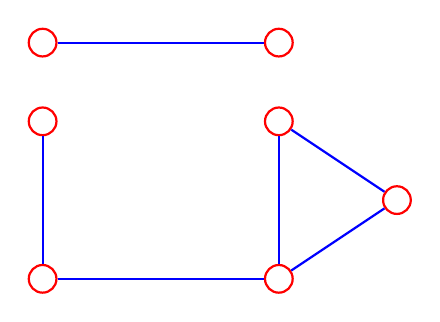
\begin{tikzpicture} % lagt till
    \tikzstyle{vertex}=[circle, minimum size=10pt, draw=red, thick]
    \tikzstyle{edge}=[-, thick, draw=blue]
    
    \node[vertex] (v1) at (0,4) {};
    \node[vertex] (v2) at (3,4) {};
    \node[vertex] (v3) at (0,3) {};
    \node[vertex] (v4) at (3,3) {};
    \node[vertex] (v5) at (0,1) {};
    \node[vertex] (v6) at (3,1) {};
    \node[vertex] (v7) at (4.5,2) {};
    
    \draw[edge] (v1) -- (v2);
    \draw[edge] (v3) -- (v5);
    \draw[edge] (v5) -- (v6);
    \draw[edge] (v6) -- (v4);
    \draw[edge] (v6) -- (v7);
    \draw[edge] (v7) -- (v4);
    
    \end{tikzpicture}
    
    \caption[][2cm]{Ett exempel på en graf. Den är inte sammanhängande, eftersom de övre två noderna inte kan nås från de undre fem. Triangeln utgör en cykel, som är grafens enda.}
    \end{figure}
    \end{center}
    
    \begin{comment}
    \begin{figure}
        \centering
        \includegraphics[width=0.4\textwidth]{graphics/example_graph.png}
        \caption[][2cm]{Ett exempel på en graf. Den är inte sammanhängande, eftersom de övre två noderna inte kan nås från de undre fem. Triangeln utgör en cykel, som är grafens enda.}
    \end{figure}
    \end{comment}
\end{definition}

\begin{example}
    Det finns $2^{\binom{n}{2}}$ stycken etiketterade grafer på $n$ noder, eftersom det finns $\binom{n}{2}$ möjliga kanter, och vi får en graf per val av vilka kanter som skall vara med.

    Problemet med att räkna antalet oetiketterade grafer på $n$ noder är betydligt mer komplicerat. Den första idén man hade haft är kanske att det borde vara
    $$\frac{2^{\binom{n}{2}}}{n!}$$
    eftersom det borde finnas $n!$ olika sätt att sätta dit etiketterna. Problemet är att vissa grafer har symmetrier som gör att till synes olika sätt att skriva dit etiketter i själva verket ger samma etiketterade graf.

    \begin{figure}
        \centering
        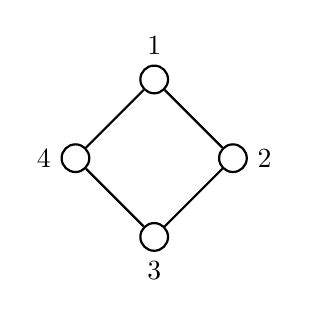
\begin{tikzpicture} % lagt till
        \tikzstyle{vertex}=[circle, minimum size=10pt, draw=black, thick]
        \tikzstyle{edge}=[-, thick, draw=black]
        \node[vertex] (v2) at (0:1cm) [label=right:2]{};
        \node[vertex] (v1) at (90:1cm) [label=above:1]{};
        \node[vertex] (v4) at (180:1cm) [label=left:4]{};
        \node[vertex] (v3) at (270:1cm) [label=below:3]{};
        \draw[edge] (v1) -- (v2);
        \draw[edge] (v2) -- (v3);
        \draw[edge] (v3) -- (v4);
        \draw[edge] (v1) -- (v4);
        \end{tikzpicture}
        \qquad
        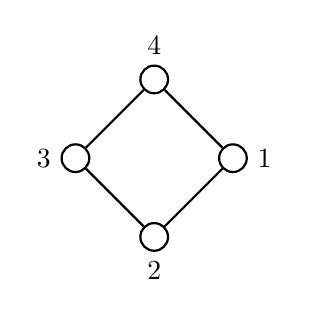
\begin{tikzpicture}
        \tikzstyle{vertex}=[circle, minimum size=10pt, draw=black, thick]
        \tikzstyle{edge}=[-, thick, draw=black]
        \node[vertex] (v1) at (0:1cm) [label=right:1]{};
        \node[vertex] (v4) at (90:1cm) [label=above:4]{};
        \node[vertex] (v3) at (180:1cm) [label=left:3]{};
        \node[vertex] (v2) at (270:1cm) [label=below:2]{};
        \draw[edge] (v1) -- (v2);
        \draw[edge] (v2) -- (v3);
        \draw[edge] (v3) -- (v4);
        \draw[edge] (v1) -- (v4);
        \end{tikzpicture}
        \caption{Två till synes olika etiketteringar av samma graf, som i själva verket är samma etikettering på grund av grafens rotationssymmetri.}
    \end{figure}

    \begin{comment}
    \begin{figure}
        \centering
        \includegraphics[width=0.5\textwidth]{graphics/counting_labelled_graphs.png}
        \caption{Två till synes olika etiketteringar av samma graf, som i själva verket är samma etikettering på grund av grafens rotationssymmetri.}
    \end{figure}
    \end{comment}

    Som tur är visar det sig att nästan alla grafer inte har någon symmetri alls, så svaret är \emph{nästan} $\frac{2^{\binom{n}{2}}}{n!}$.\sidenote[][-1.5cm]{Det här påståendet låter kanske löst i kanten, men det är faktiskt helt rigoröst. I alla fall om man ersätter ``nästan'' med att skriva att antalet är
    $$(1 + o(1))\frac{2^{\binom{n}{2}}}{n!}.$$}
\end{example}

\begin{definition}
    \begin{marginfigure}
        \centering
        \begin{tikzpicture} % lagt till
            \tikzset{
                every node/.style={
                draw, circle, inner sep=0pt, minimum width=10pt, draw=red
                }
            }
        \node {}
            child {  node {}
                child { node {}}}
            child { node {}
                child { node{}}
                child { node{}}
                }
            child { node {}}
            edge from parent [blue]
            ;
        \end{tikzpicture}    
        %\includegraphics[width=0.6\textwidth]{graphics/example_tree.png}
        \caption{Ett träd med sju noder och sex kanter.}
    \end{marginfigure}

    Ett \emph{träd} är en sammanhängande graf utan cykler. Ett \emph{rotat} träd är ett träd med en specifik nod utpekad som dess rot.\sidenote[][]{Så om trädet är oetiketterat kan vi alltså se vilken nod som är roten, men resten av noderna kan vi inte se skillnad på, bara vilka som hänger ihop med vilka med kanter.} I ett rotat träd har varje nod utom roten själv en granne som är närmre roten än sig\sidenote[][]{Eller är roten.}, vilken vi kallar dess \emph{förälder}. Alla dess andra grannar kallar vi dess \emph{barn} och två noder med samma förälder kallar vi för \emph{syskon}. En nod utan barn kallar vi för ett \emph{löv}, och en nod som inte är ett löv kallar vi för \emph{intern}. Man kan även säga att djupet för en nod är antalet steg från rotnoden till noden. Rotnoden är på djup 0, dess barn är på djup 1, osv. 

    Ifall det spelar roll i vilken ordning vi ritat noderna kallar vi trädet \emph{ordnat}, se figur \ref{fig:distinct_only_as_ordered}.

    \begin{marginfigure}
        \centering
        % lagt till
        \begin{tikzpicture} % potential corrections: bigger angle between edges of first to second generation
            \tikzset{
                every node/.style={
                draw, circle, inner sep=0pt, minimum width=10pt, draw=red
                }
            }
        \node (a) {}
            [sibling distance = 1.5cm]
            child { node {}
            [sibling distance = 1.cm]
                child { node {}}
                child {node{}}}
            child { node {}}
            edge from parent [blue]
            ;
        \node at ([xshift=2.5cm]a) {}
            [sibling distance = 1.5cm]
            child { node {}}
            child { node {}
            [sibling distance = 1cm]
                child { node{}}
                child{ node{}}
                }
            edge from parent [blue]
            ;
        \end{tikzpicture}        
    
        %\includegraphics[width=0.8\textwidth]{graphics/ordered_versus_unordered_trees.png}
        \caption{Två träd som är olika varandra som ordnade träd, men samma träd som oordnade träd.}
        \label{fig:distinct_only_as_ordered}
    \end{marginfigure}
\end{definition}

\begin{example}
    Träd kan verka abstraka och men de manifesteras daligen i vardagliga sammanhang. \\Alla typer av slutspel (kvartsfinal, semifinal och final) är representerade av ett träd. \\Även din dators filstruktur kan representeras av ett träd.\\ Om du tar upp terminalen för MacOS, eller din command prompt på Windows kommer du se att du är i roten av din dator.\\ Om du kör kommandot $ls$ kommer du sedan se dina huvudmappar som datorn är indelad i.\\De kan ses som de noder i trädet med djup 1. Du kan sedan gå in i dessa mappar med kommandot $cd$ $dinmapp$ och se barnen till den noden, osv. Det blir förhoppningsvis tydligt att se hur datorns alla filer är strukturerade som ett träd. \\  
\end{example}

\begin{definition}
    Ett träd i vilket alla noder antingen har två eller noll barn kallas för ett \emph{binärt} träd.
\end{definition}

\begin{example}
    Binära träd är intressanta att studera, framförallt binära sökträd som är en typ av binärt träd. Här kräver man en viss typ av ordning av noderna som säger att nodens vänstra barn ska vara mindre än sin förälder och att nodens högra barn ska vara större än sin förälder. 

    \begin{figure}
        \centering
        \includegraphics{graphics/F8/Bts.jpeg}
        \caption{Ett binärt sökträd med roten 8, storlek 9 och djup 3, hämtat från https://en.wikipedia.org/wiki/Binary\_search\_tree}
        \label{fig:Bts}
    \end{figure}

Binära sökträd uppfans på 60-talet för att lösa ett problem kring att effektivisera lagring av etiketterad data. Att hitta, sätta in och ta bort något ur ett binärt sökträd är i genomsnitt mycket snabbare än på ett vanligt binärt träd. Binära sökträd har många användningsområden, bland annat är det ett bra sätt att lösa indexering av data i stora databaser.

\end{example}

\section{Ännu fler saker som räknas av Catalantalen}

Låt oss nu återse en gammal vän, Catalantalen.

\begin{proposition}
    Antalet rotade ordnade binära oetiketterade träd med $n$ stycken interna noder ges av Catalantalen.

    \begin{proof}
        Vi kan dela upp ett sådant träd i två mindre träd genom att helt enkelt ta bort roten, och låta dess två barn vara rötter i två mindre träd.

        \begin{figure}
            \centering        
            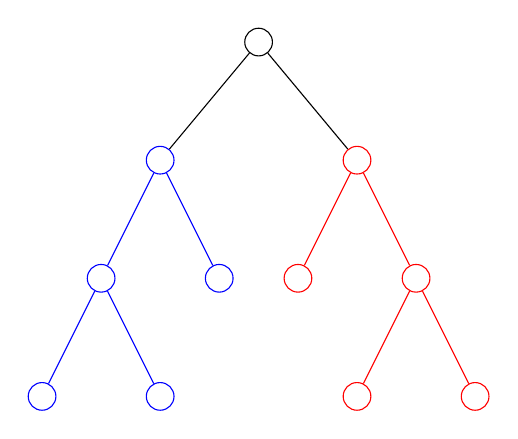
\begin{tikzpicture} % lagt till
                \tikzset{
                    every node/.style={
                    draw, circle, inner sep=0pt, minimum width=10pt
                    }
                }
            \node {} [sibling distance = 2.5cm]
                child {node [blue]{} [sibling distance = 1.5cm]
                    child [blue] {node{}
                        child {node{}}
                        child {node{}}
                        }
                    child [blue] {node{}}
                    }
                child {node [red]{}
                [sibling distance = 1.5cm]
                    child [red] {node{}}
                    child [red] {node{}
                        child {node{}}
                        child {node{}}
                        }
                    }
                ;
            \end{tikzpicture}
            
            %\includegraphics[width=0.5\textwidth]{graphics/RUBOTree_division.png}
            \caption[][1.5cm]{Ett rotat ordnat binärt oetiketterat träd, med uppdelningen av det i två mindre träd av samma typ, ett rött och ett blått.}
        \end{figure}

        Alltså gäller det, om $t_n$ betecknar antalet sådana träd, att
        $$t_{n+1} = \sum_{k=0}^{n} t_k t_{n-k},$$
        eftersom vi kan skapa oss ett sådant träd med $n+1$ noder genom att först rita roten, och sedan fästa ett träd med $k$ interna noder till vänster och ett med $n-k$ interna noder till höger. Eftersom roten själv är intern har vi då $k + n - k + 1 = n + 1$ interna noder.
    \end{proof}
\end{proposition}

I själva verket räknas också godtyckliga oetiketterade ordnade träd av Catalantalen, utan något krav på att de skall vara binära.

\begin{proposition}
    Antalet rotade ordnade oetiketterade träd på $n+1$ noder ges av Catalantalen.\sidenote[][]{Notera att vi här räknar \emph{alla} noder, inte bara de interna, som vi gjorde för de binära träden.}

    \begin{proof}
        Vi bevisar detta genom att uppvisa en bijektion med sätt att skriva $n$ matchande par av parenteser.

        Så, givet ett rotat ordnat oetiketterat träd på $n+1$ noder, numrera dess löv från höger till vänster.

        \begin{figure}
            \centering
            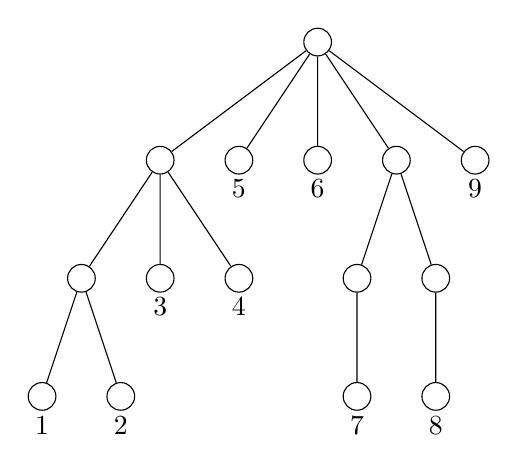
\begin{tikzpicture} % lagt till
                \tikzset{
                    every node/.style={
                    draw, circle, inner sep=0pt, minimum width=10pt
                    }
                }
            \node {} [sibling distance = 1cm]
                child {node{} 
                    child {node{}
                        child {node[label=below:1]{}}
                        child {node[label=below:2]{}}
                        }
                    child {node[label=below:3]{}}
                    child {node[label=below:4]{}}
                    }
                child {node[label=below:5]{}}
                child {node[label=below:6]{}}
                child {node{}
                    child{node{}
                        child{node[label=below:7]{}}
                        }
                    child{node{}
                        child{node[label=below:8]{}}
                        }
                    }
                child {node[label=below:9]{}}
                ;
            \end{tikzpicture}
            
            %\includegraphics[width=0.6\textwidth]{graphics/rooted_ordered_general_tree_with_leaf_labels.png}
            \caption{Ett rotat ordnat oetiketterat träd, med dess löv numrerade från vänster till höger.
            
            I vår algoritm för att omvandla detta träd till en parentetisering blir uttrycket, innan vi ersatt talen med $()$,
            $$((12)34)56((7)(8))9.$$}
        \end{figure}

        Skriv sedan upp talen $12\ldots k$ på rad, och skriv i parenteser på följande vis: För varje intern nod, förutom roten, skriv ett par parenteser runt alla de tal som motsvarar löv under noden. Ersätt sedan varje av talen med ett tomt par av parenteser, $()$. Detta ger en parentetisering med precis $n$ par av parenteser.

        För att återhämta ett träd från en parentetisering, börja med att rita en nod för varje $()$. Sedan, för varje grupp av noder som ligger i samma par av parenteser, rita en gemensam förälder för dem. Till slut, rita dit roten, och koppla den till varje par av parenteser som inte har någon parentes runt sig.
    \end{proof}
\end{proposition}

\section{Cayleys formel}

Vi har alltså lyckats räkna två specifika sorters träd. Kan vi räkna träd mer generellt?

\begin{theorem}
    Det finns
    $$n^{n-2}$$
    stycken etiketterade träd med $n$ noder.
\end{theorem}

För att förstå detta resultat, låt oss börja med att räkna de första små fallen. Vi kollar på \emph{oetiketterade} träd, och räknar hur många sätt vi kan sätta etiketter på dem.

\begin{figure}
    \centering
    \begin{itemize} % lagt till
        \item[$n=1:$] \qquad
        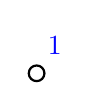
\begin{tikzpicture}
        \tikzstyle{vertex}=[circle, minimum size=1pt, inner sep=2pt, draw=black, thick]
        \tikzstyle{edge}=[-, thick, draw=black]
        
        \node[vertex] (v1) at (0,5) [label={[text=blue]80:$1$}]{};
        
        %\draw[edge] (v1) -- (v2);
        \end{tikzpicture}\\
        
        \item[$n=2:$] \qquad
        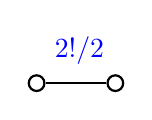
\begin{tikzpicture}
        \tikzstyle{vertex}=[circle, minimum size=1pt, inner sep=2pt, draw=black, thick]
        \tikzstyle{edge}=[-, thick, draw=black]
        
        \node[vertex] (v1) at (0,0) {};
        \node[vertex] (v2) at (1,0) [label={[text=blue]100:$2!/2$}]{};
        \draw[edge] (v1) -- (v2);
        \end{tikzpicture}\\
        
        \item[$n=3:$] \qquad
        \begin{tikzpicture}
        \tikzstyle{vertex}=[circle, minimum size=1pt, inner sep=2pt, draw=black, thick]
        \tikzstyle{edge}=[-, thick, draw=black]
        
        \node[vertex] (v1) at (0.5,0.5) {};
        \node[vertex] (v2) at (0,0) {}; 
        \node[vertex] (v3) at (1,0) [label={[text=blue]88:$3$}]{};
        \draw[edge] (v1) -- (v2);
        \draw[edge] (v1) -- (v3)
        \end{tikzpicture}\\
        
        \item[$n=4:$] \qquad
        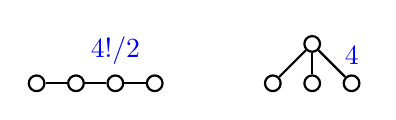
\begin{tikzpicture}
        \tikzstyle{vertex}=[circle, minimum size=1pt, inner sep=2pt, draw=black, thick]
        \tikzstyle{edge}=[-, thick, draw=black]
        
        \node[vertex] (v1) at (0,0) {};
        \node[vertex] (v2) at (0.5,0) {}; 
        \node[vertex] (v3) at (1,0) [label={[text=blue]90:$4!/2$}]{};
        \node[vertex] (v4) at (1.5,0) {};
        \draw[edge] (v1) -- (v2);
        \draw[edge] (v2) -- (v3);
        \draw[edge] (v3) -- (v4);
        
        \node[vertex] (v5) at (3,0) {};
        \node[vertex] (v6) at (3.5,0) {}; 
        \node[vertex] (v7) at (4,0) [label={[text=blue]89:$4$}]{};
        \node[vertex] (v8) at (3.5,0.5) {};
        \draw[edge] (v5) -- (v8);
        \draw[edge] (v6) -- (v8);
        \draw[edge] (v7) -- (v8);
        \end{tikzpicture}\\
        
        \item[$n=5:$]
        \item[]\qquad\qquad\;
        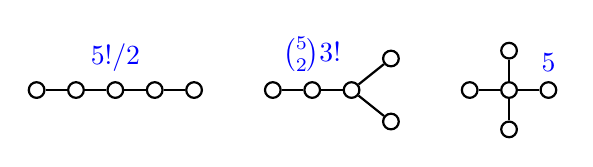
\begin{tikzpicture}
        \tikzstyle{vertex}=[circle, minimum size=1pt, inner sep=2pt, draw=black, thick]
        \tikzstyle{edge}=[-, thick, draw=black]
        
        \node[vertex] (v1) at (0,0) {};
        \node[vertex] (v2) at (0.5,0) {}; 
        \node[vertex] (v3) at (1,0) [label={[text=blue]90:$5!/2$}]{};
        \node[vertex] (v4) at (1.5,0) {};
        \node[vertex] (v5) at (2,0) {};
        \draw[edge] (v1) -- (v2);
        \draw[edge] (v2) -- (v3);
        \draw[edge] (v3) -- (v4);
        \draw[edge] (v4) -- (v5);
        
        \node[vertex] (v5) at (3,0) {};
        \node[vertex] (v6) at (3.5,0) {}; 
        \node[vertex] (v7) at (4,0) [label={[text=blue]95:$\binom{5}{2} 3!$}]{};
        \node[vertex] (v8) at (4.5,-0.4) {};
        \node[vertex] (v9) at (4.5,0.4) {};
        \draw[edge] (v5) -- (v6);
        \draw[edge] (v6) -- (v7);
        \draw[edge] (v7) -- (v8);
        \draw[edge] (v7) -- (v9);
        
        \node[vertex] (v10) at (5.5,0) {};
        \node[vertex] (v11) at (6,0.5) {};
        \node[vertex] (v12) at (6,0) {};
        \node[vertex] (v13) at (6,-0.5) {};
        \node[vertex] (v14) at (6.5,0) [label={[text=blue]90:$5$}]{};
        \draw[edge] (v10) -- (v12);
        \draw[edge] (v11) -- (v12);
        \draw[edge] (v13) -- (v12);
        \draw[edge] (v14) -- (v12);
        
        \end{tikzpicture}
    \end{itemize}
        
    %\includegraphics[width = \textwidth]{graphics/counting_tree_labellings.png}
    \caption{Oetiketterade grafer med $n$ noder, för $n = 1,\ldots,5$, med antalet sätt att sätta etiketter på varje i blått.}
\end{figure}

Sätten vi får dessa antal är, per värde på $n$:
\begin{enumerate}
    \item Att det bara finns ett sätt att skriva en etta på den enda noden är uppenbart.
    \item Vi kan välja vilken permutation som helst av $[2]$ att skriva på noderna, men grafen har en speglingssymmetri, så att skriva etiketterna i motsatt ordning ger samma träd. Alltså $\frac{2!}{2}$.
    \item Vi kan se vilken nod som är den mellersta, men vi kan inte se skillnad på de två yttre. Alltså är det enda val vi kan göra det av vilket tal vi skriver på den mellersta, vilket vi kan välja på tre sätt.
    \item För den första av våra två oetiketterade grafer kan vi skriva vilken permutation av $[4]$ vi vill, men återigen har vi en speglingssymmetri, så att skriva den baklänges ger oss samma etikettering. Alltså $\frac{4!}{2}$.
    
    För den andra är vi i samma situation som vi var i för $n=3$ -- vi kan se vilken nod det är som har mer än en granne, men vi kan inte se skillnad på de andra. Alltså är det enda valet vi har vilken etikett just den särskilda noden får, vilket vi kan göra på $4$ sätt.
    \item Vi får $\frac{5!}{2}$ av samma speglingssymmetri-skäl som innan, och för den tredje av våra grafer får vi $5$ eftersom vi åter har en särskild nod och resten kan vi inte se skillnad på.
    
    För den mellersta av våra tre oetiketterade träd kan vi se skillnad på de tre noderna i svansen till vänster, men de två som sticker ut åt höger kan vi inte se skillnad på. Så för att etikettera denna väljer vi två etiketter för de talen, vilket vi kan göra på $\binom{5}{2}$ sätt, och sedan är varje permutation av de återstående tre etiketterna faktiskt en distinkt etikettering, så vi kan välja $3!$ sätt att fullfölja vår etikettering. Så vi har totalt $\binom{5}{2}3!$ sätt att göra detta på.
\end{enumerate}

Så vi ser i alla fall att vår formel gäller för $n$ upp till fem. Vi väljer att ge två bevis för denna sats. Det första är av Prüfer, och ger en bijektion mellan etiketterade träd och en enklare mängd.

\begin{proof}[Prüfers bevis av Cayleys formel (1918)]
    Vi vill visa på en bijektion mellan mängden av etiketterade träd på $n$ noder och mängden av ord av längd $n-2$ ur alfabetet $[n]$. Att den senare mängden har rätt antal element vet vi sedan innan, så om vi kan hitta en bijektion är vi klara.

    Vi börjar med att berätta hur vi skapar vårt ord givet ett etiketterat träd.\sidenote[][-0.5cm]{Detta ord kallas för trädets \emph{Prüferkod}.} Vi letar upp det löv\sidenote[][]{Strikt sett har vi hittills bara definierat \emph{löv} för rotade träd -- och de träd vi studerar här har ju ingen rot-nod. Med ``löv'' menar vi här ``nod med bara en granne''.} som har lägst etikett, skriver dess etikett som första bokstav i vårt ord, och tar sedan bort noden ur trädet.

    \begin{figure}
        \centering
        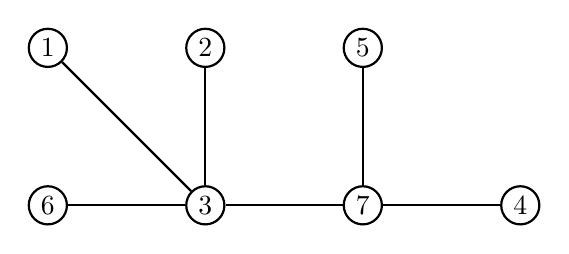
\begin{tikzpicture} % lagt till
        \tikzstyle{vertex}=[circle, minimum size=12pt, inner sep=2pt, draw=black, thick]
        \tikzstyle{edge}=[-, thick, draw=black]
        
        
        \node[vertex] (v1) at (0,2) {$1$};
        \node[vertex] (v2) at (2,2) {$2$};
        \node[vertex] (v5) at (4,2) {$5$};
        \node[vertex] (v6) at (0,0) {$6$};
        \node[vertex] (v3) at (2,0) {$3$};
        \node[vertex] (v7) at (4,0) {$7$};
        \node[vertex] (v4) at (6,0) {$4$};
        
        \draw[edge] (v1) -- (v3);
        \draw[edge] (v2) -- (v3);
        \draw[edge] (v3) -- (v6);
        \draw[edge] (v3) -- (v7);
        \draw[edge] (v5) -- (v7);
        \draw[edge] (v4) -- (v7);
        \end{tikzpicture}
        
        %\includegraphics[width=0.75\textwidth]{graphics/prufer_code_tree_example.png}
        \caption[][1.25cm]{Ett etiketterat träd med Prüferkod $33773$.}
    \end{figure}

    Vi upprepar denna process -- letar upp det löv i det resulterande trädet som har lägst etikett (och notera att vi, när vi tar bort ett löv, ibland kommer göra en nod som innan var intern till ett löv), skriver den etiketten på slutet av ordet, och tar bort lövet. Processen fortsätter tills vi bara har två noder kvar.

    För att gå från en Prüferkod till en etiketterad graf använder vi följande algoritm, som konstruerar ett etiketterat träd givet en Prüferkod $a_1a_2\ldots a_{n-2}$.

    \begin{algorithm}
        \caption{Konstruktion av träd från Prüferkoder}\label{alg:constr_tree_from_prufer_code}
        \begin{algorithmic}
            \State Låt $G$ vara en graf med $n$ noder, med etiketter $1, 2, \ldots, n$, men utan kanter
            \State Skapa en lista i $L$ som inehåller etikterna i $G$ i storlkesordning, alltså $1, 2 \ldots, n$.
            \State Skapa även listan $P$ som innehåller Prüferkoden
            \While P (Loopen kör tills det inte finns något kvar i $P$)
            \State Låt $l$ vara det minsta elementet i $L$ som inte finns med i $P$
            \State Låt $p$ vara det första elementet i $P$
            \State Rita en kant i $G$ mellan $l$ och $p$ 
            \State $L = L - l$
            \State $P = P - p$
            \EndWhile
            \State Rita en kant i $G$ mellan de två elementen som finns kvar i $L$\\
            \Return $G$
        \end{algorithmic}
    \end{algorithm}


    Det tar en stund att förstå vad den här algoritmen faktiskt gör\sidenote[][-1cm]{En fördel med föreläsningar över text är att man faktiskt kan genomföra algoritmen på ett konkret exempel, för att illustrera den, men en text måste så klart vara statisk. Sitter du hemma och läser föreslår jag att du prövar att göra algoritmen för hand på någon eller några Prüferkoder, för att få en känsla för vad som pågår.}, men efter en stunds kontemplation ser man att vad den gör är att den lägger till kanterna i precis den ordning som de försvann när vi skapade Prüferkoden.

   

    \begin{figure}
        \centering
        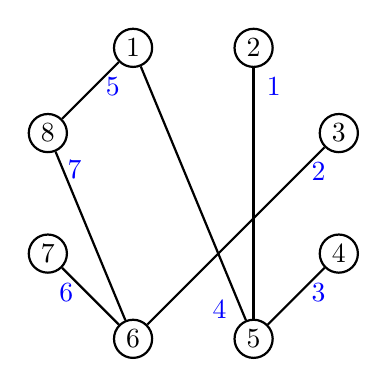
\begin{tikzpicture} % lagt till
        \tikzstyle{vertex}=[circle, minimum size=5pt, inner sep=2pt, draw=black, thick]
        \tikzstyle{edge}=[-, thick, draw=black]
        
        \node[vertex] (v1) at (112.5:2cm) [label={[text=blue]260:5}] {$1$};
        \node[vertex] (v2) at (67.5:2cm) [label={[text=blue]280:1}]{$2$};
        \node[vertex] (v3) at (22.5:2cm) [label={[text=blue]260:2}]{$3$};
        \node[vertex] (v4) at (337.5:2cm) [label={[text=blue]260:3}]{$4$};
        \node[vertex] (v5) at (292.5:2cm) [label={[text=blue]150:4}]{$5$};
        \node[vertex] (v6) at (247.5:2cm) {$6$};
        \node[vertex] (v7) at (202.5:2cm) [label={[text=blue]275:6}]{$7$};
        \node[vertex] (v8) at (157.5:2cm) [label={[text=blue]300:7}]{$8$};
        
        \draw[edge] (v1) -- (v5);
        \draw[edge] (v1) -- (v8);
        \draw[edge] (v2) -- (v5);
        \draw[edge] (v3) -- (v6);
        \draw[edge] (v4) -- (v5);
        \draw[edge] (v6) -- (v7);
        \draw[edge] (v6) -- (v8);
        \end{tikzpicture}
        
        %\includegraphics[width=0.6\textwidth]{graphics/tree_from_prufer_code.png}
        \caption{Ett träd skapat från Prüferkoden $565186$. I blått har vi markerat i vilket steg i algoritmen varje kant lades till -- lägg märke till att detta är precis ordningen i vilken de \emph{tas bort} om vi skapar Prüferkoden för detta trädet.} 
    \end{figure}

    Den första kanten att ritas kommer att gå mellan det första lövet som tas bort och dess granne, den andra går mellan andra lövet att tas bort och dess granne, och så vidare -- ända fram tills den sista kanten vi lägger till, som går mellan de två kvarvarande noderna när vi byggde Prüferkoden. Alltså kommer denna algoritmen precis att rekonstruera grafen vi började med, vilket bevisar att vi faktiskt har en bijektion, och satsen följer.

    Detaljerad förklaring varför just dettta träd som figuren visar kommer från Prüferkoden $565186$ : Vi tittar på den lägsta etiketten med endast en granne, det är löv nr 2 (löv nr 1 har flera grannar). Löv nr 2 sträcker sig till löv nr 5 så 5 blir första siffran i koden. Denna nod mellan 2 och 5 strycks nu. Återigen, vi tittar på det löv med lägst etikett, detta är nu 3, 3 sträcker sig till 6 så 6 blir nästa siffra i koden. Nästa lägsta löv med endast en granne är löv nr 4, denna sträcker sig till 5 så 5 blir nästa siffra i koden. Nu har löv nr 5 endast en kant till löv nr 1 eftersom de andra 2 kanterna är strukna, nästa siffra blir därför 1. Nu har löv nr 1 en granne och det är 8, 8 blir nästa siffra i koden. Till sist sträcker sig löv nr 7 till löv nr 6, 6 blir därför sista siffran i koden. Vi får helt riktigt koden $565186$.

    
\end{proof}

\section{Ett alternativt bevis av Cayleys formel}

Det bevis vi just gav av Cayleys formel är visserligen elegant, men det är inte det enda beviset av denna sats. Det finns åtskilliga andra bevis -- inte bara med hjälp av bijektioner, utan också med rekursioner, och ett klassiskt bevis som använder determinanter och Kirchhoffs matris-träd-sats.

Beviset vi skall ge nu använder inga avancerade metoder alls, inte ens en bijektion, utan är bara ett helt vanligt ``räkna på två sätt''-bevis. I boken jag tog det från
\sidenote[][-1.5cm]{Beviset är av Jim Pitman, men boken är \emph{Proofs from the Book}. Den får detta namn från hur Erd\H{o}s brukade påstå att Gud hade en bok som innehöll alla de vackraste bevisen. (Kanske en väldigt infantil version av de medeltida teologernas idéer om matematiken som Guds ordning i Hans skapelseverk?) 

Hela idén om ``boken'' är egentligen lite märklig, med tanke på att Erd\H{o}s var ateist -- om än av typen som är arg på Gud för Hans påstådda ickeexistens.

Själva boken (den jag tog beviset ur, alltså) är, för övrigt, inte så särskilt bra, i min mening. Den gör bevisen mer komplicerade än de behöver vara, och har ett lite udda urval. Herren har definitivt en bättre bok, även om allvetande kanske får anses som fusk när man letar efter bevis.} 
beskrivs detta som ``det vackraste beviset av dem alla'', men personligen föredrar jag nog Prüfers bevis, som inte ens var med på deras lista.

För att kunna ge detta bevis behöver vi definiera några fler koncept.

\begin{definition}
    En \emph{riktad} graf är en graf där varje kant har en utpekad start- och slutnod. Vi tänker oss kanterna som pilar som pekar från start till slut.

    Det finns ett uppenbart sätt att omvandla ett rotat träd till ett \emph{riktat} träd\sidenote[][0.4cm]{Alltså ett träd som har riktade kanter.} genom att ge varje kant den riktning som pekar bort från roten, och vice versa kan vi, för ett riktat träd med konsistenta riktningar på kanterna göra om det till ett rotat oriktat träd.
\end{definition}

\begin{definition}
    En graf $H$ med noder $V_H$ och kanter $E_H$ är en \emph{delgraf} till en graf $G = (V_G, E_G)$ om $V_H\subseteq V_G$ och 
    $$E_H \subseteq \left\{\{u,v\} \in E_G: u, v \in V_H\right\}.$$
    För att skapa oss en delgraf till $G$ tar vi alltså någon delmängd till dess noder, och tar sedan någon delmängd av kanterna mellan dessa noder.

    Om graferna är riktade kräver vi att de skall ha samma riktning i $G$ som i $H$. Om de är etiketterade kräver vi att etiketterna skall matcha i $H$ och $G$.
\end{definition}

\begin{definition}
    En \emph{skog} är en graf sådan att varje sammanhängande komponent är ett träd. Eller ekvivalent kan vi säga att det är en graf utan cykler.

    En \emph{rotad} skog är en skog med ett val av rot för varje träd i skogen.
\end{definition}

\begin{proof}[Alternativt bevis av Cayleys sats]
    Låt $\mathcal{F}_{n,k}$ beteckna mängden av rotade skogar med $n$ noder, som består av $k$ träd. Alltså är $\mathcal{F}_{n,1}$ antalet rotade träd -- om vi kan räkna dem är vi klara, eftersom vi vet att det finns precis $n$ val av rot, så $\frac{\abs{T_{n,1}}}{n}$ är talet vi söker.

    Vi säger att en skog $F'$ \emph{ligger i} en annan skog $F$ om $F'$ är en delgraf till $F$ när vi betraktar dem som riktade träd.\sidenote[][-0.3cm]{Vi har ju inte definierat vad vi menar med att ett \emph{rotat} träd skulle vara en delgraf till ett annat. För att vara tydliga betyder detta att vi \emph{inte} kräver att roten till ett träd i $F'$ också är rot till det större träd det ligger i i $F$.}

    \begin{figure}
        \centering   
        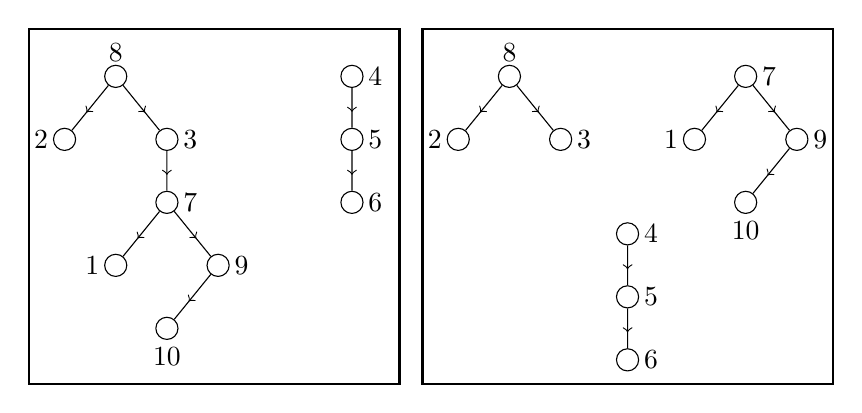
\begin{tikzpicture}[level distance=8mm] % lagt till
            \tikzset{
                every node/.style={
                draw, circle, inner sep=0pt, minimum width=8pt
                },
                ->-/.style={decoration={
                markings,
                mark=at position #1 with {\arrow{>}}},postaction={decorate}},
                edge from parent/.style={
                draw, ->-=.6
                }
            }
        \node (a) [label=above:8]{} [sibling distance = 1.3cm]
            child {node[label=left:2]{}} 
            child {node[label=right:3]{}
                child{node[label=right:7]{}
                child{node[label=left:1]{}}
                child{node[label=right:9]{}
                    child{node[label=below:10]{}}
                    child [ missing ]}}}
            ;
        \node at ([xshift=3cm]a) [label=right:4]{}
            child {node [label=right:5]{}
            child {node [label=right:6]{}}}
            ;
            \draw[black,thick] ($(a.north west)+(-1,0.5)$)  rectangle ($(a.south east)+(3.5,-3.8)$);
        
        \node (b) at ([xshift=5cm]a) [label=above:8]{} [sibling distance = 1.3cm]
            child {node[label=left:2]{}} 
            child {node[label=right:3]{}
                }
            ;
            \draw[black,thick] ($(b.north west)+(-1,0.5)$)  rectangle ($(b.south east)+(4,-3.8)$);
        \node at ([xshift=8cm]a) [label=right:7]{} [sibling distance = 1.3cm]
            child{node[label=left:1]{}}
            child{node[label=right:9]{}
                child{node[label=below:10]{}}
                child [ missing ]}
                ;
        \node at ([xshift=6.5cm, yshift=-2cm]a) [label=right:4]{} [sibling distance = 1.3cm]
            child {node [label=right:5]{}
            child {node [label=right:6]{}}}
            ;
        \end{tikzpicture}

        
        %\includegraphics[width=0.95\textwidth]{graphics/rooted_forest_subforest.png}
        \caption[][1.2cm]{Två rotade skogar $F_2$ till vänster och $F_3$ till höger, betraktade som riktade träd. Notera att $F_3$ ligger i $F_2$.}
        \label{fig:two_rooted_forests}
    \end{figure}

    Nyckelidén i vårt bevis är \emph{klyvande följder} av rotade skogar. Vi säger att en följd $F_1, F_2,\ldots, F_k$ av rotade skogar på $n$ noder är \emph{klyvande} om varje $F_i$ består av $i$ stycken träd, och $F_{i}$ innehåller $F_{i+1}$ för varje $i$.

    Låt nu $F_k \in \mathcal{F}_{n,k}$ vara en fix skog, och beteckna
    \begin{itemize}
        \item antalet rotade \emph{träd} som innehåller $F_k$ med $N(F_k)$, och
        \item antalet klyvande följder som slutar med $F_k$ med $N^*(F_k)$.
    \end{itemize}

    Notera nu att om vi tar $k = n$ finns det bara ett val för $F_k$, nämligen skogen av $n$ stycken träd, där varje träd bara är en enda nod -- och \emph{varje} rotat träd på $n$ noder innehåller denna skog. Alltså är $N(F_n)$ helt enkelt antalet rotade träd, vilket ju är vad vi vill räkna.

    Så om vi kan hitta en formel för $N(F_k)$ är vi klara. Vi gör detta genom att räkna $N^*(F_k)$ på två olika sätt. Först går vi från $F_k$ till $F_1$, och sedan i motsatt riktning.

    Givet ett $F_k$, hur många val har vi av av $F_{k-1}$? Eftersom $F_{k-1}$ ska ha ett träd färre, måste vi foga ihop två träd med en kant. Den här kanten kan utgå från vilken nod som helst, och skall träffa en av de $k-1$ rötterna till andra träd än det träd noden själv är i.\sidenote[][]{Den måste träffa en rot för att riktningen på kanterna skall förbli konsekvent -- om den träffade en ickerot hade vi fått en nod som är slutnod för två kanter, och alltså har två föräldrar, vilket vi inte tillåter.} I figur \ref{fig:two_rooted_forests} kan vi till exempel få $F_2$ från $F_3$ genom att rita dit en kant från $3$ till $7$, som är roten för sitt träd.

    Vi kan alltså välja $F_{k-1}$ givet $F_k$ på $n(k-1)$ sätt. Precis samma argument ger att vi kan välja $F_{k-2}$ givet $F_{k-1}$ på $n(k-2)$ sätt, och så vidare. Så totalt kan vi välja vår följd $F_k, F_{k-1}, \ldots, F_1$ på
    $$N^*(F_k) = n^{k-1}(k-1)!$$
    sätt.

    Så till den andra riktningen -- givet $F_k$ finns det, per definition, precis $N(F_k)$ val av $F_1$, eftersom $F_1$ skall vara något rotat träd som innehåller $F_k$. Vi ser enkelt att det är precis $k-1$ kanter som ligger i $F_1$ men inte i $F_k$ -- när vi räknade i motsatta riktningen är det dessa vi lade till.

    Tar vi bort en av dessa kanter klyver vi $F_1$ och får en skog $F_2$, tar vi bort en till klyver vi ytterligare ett träd och får $F_3$, och så vidare -- och varje klyvande följd $F_1, F_2, \ldots, F_k$ med fixt $F_1$ och $F_k$ kan fås på detta vis.

    Uppenbarligen är antalet sätt att välja en ordning att ta bort de $k-1$ kanterna i precis $(k-1)!$, så vad vi har visat är att
    $$N^*(F_k) = N(F_k)(k-1)!$$
    vilket tillsammans med vårt andra sätt att räkna $N^*(F_k)$ ger oss att
    $$N(F_k) = n^{k-1}.$$

    Vi observerade innan att $N(F_n)$ är lika med det totala antalet rotade träd, och eftersom det finns $n$ sätt att välja roten till ett träd är talet vi letar efter alltså
    $$\frac{N(F_n)}{n} = \frac{n^{n-1}}{n} = n^{n-2}$$
    såsom önskat.
\end{proof}

\section{Övningar}

\begin{xca}
    Bevisa att ett träd alltid har $\abs{E} = \abs{V} - 1$.
\end{xca}
\begin{solution}\\
    Vi bevisar detta med ett induktionsbevis. \\
    Basfallet blir när $\abs{V} = 1$ vilket representerar trädet med bara en nod och inga kanter. I det fallet har vi: $1-1=0=\abs{E}$\\
    Vår induktionshypotes är att ett träd med $\abs{V}-1$ noder har $\abs{E}-2$ kanter. Nu lägger vi till en nod och ser att\\
    \begin{equation*}
        \abs{V} &= \abs{V} - 1 + 1 \stackrel{IH}{=} \abs{E}-2 +1 = \abs{E} - 1
    \end{equation*}
    När vi lägger till en nod måste vi lägga till en kant för att ett träd måste vara sammanhängande. Man kan inte lägga till en kant i trädet vi började med i induktionshypotesen för att man skulle få en cykel annars (dvs det skulle inte längre vara ett träd). Alltså går kanten från en nod i gamla trädet till nya noden, dvs det kan inte finns en cykel. Vi har skapat ett nytt träd.


    \begin{comment} % användes inte
    1. Lösning: Vi bevisar detta med ett induktionsbevis. \\ Basfallet blir när $\abs{E} = 0$ vilket, representerar trädet med bara en \\nod och inga kanter.
    Vi testar och ser om det håller för basfallet:\\
    $0 = \abs{V} - 1$\\
    $0 = 1 - 1 $\\
    $0 = 0$\\
    Basallet håller så vi går vidare till induktionsdelen. \\
    Vi ska bevisa att om vi antar att $\abs{E} = \abs{V} -1$ stämmer så ska även $\abs{E}' +1 = \abs{V}' + 1 - 1$ hålla, alltså trädet med en extra nod. Vi kallar det trädet för $\abs{T}' = \abs{T} + v$. Om vi lägger till en nod måste vi även dra en kant till den noden, så antalet kanter i $\abs{T}'$ är lika med antalet kanter i $\abs{T} + e$, alltså är $\abs{E}' = \abs{E} + 1$. 

    Lite tydligare uppstält får vi alltså att\\ $\abs{T}' = \abs{T} + v$\\$\abs{E}' = \abs{E} + 1$\\$\abs{V}' = \abs{V} + 1$. Så om vi antar att $\abs{E} = \abs{V} -1$ stämmer och sätter in $\abs{E}' och \abs{V}'$ får vi att \\$\abs{E}' - 1 = \abs{V}' - 1 - 1$\\$\abs{E}' = \abs{V}' - 1$ och vi är på samma form som urpsungsformeln. Vilket var det som skulle bevisas. 
    \end{comment}
\end{solution}

\begin{xca}
    Överväg följande skiss av ett oetiketterat träd med $1 + i + j + k$ noder:
    \begin{figure}
        \centering
        \includegraphics[width=0.8\textwidth]{graphics/exercise_label_unlabelled_tree.png}
        \caption{Skiss av ett oetiketterat träd.}
    \end{figure}

    Hur många olika sätt finns det att sätta etiketter på detta träd?\sidenote[][-1.1cm]{Vi resonerade om detta för några små träd precis efter att vi introducerade Cayleys formel, men här har vi alltså ett mer generellt fall.} Ge en formel som gäller för alla $i, j, k = 0, 1, 2,\ldots$.\sidenote[][]{Finns det några specialfall för särskilda kombinationer av värden på $i$, $j$, och $k$?} 

    
\end{xca}



    
\begin{solution}
    
    
Vi kan börja att titta längst till vänster på noderna i. Vi ska nu välja i noder av alla noder. Vi får alltså: 

$${\binom{i+1+j+k}{i}}$$ olika sätt att göra det på. Sedan kan vi titta till höger i figuren. Vi ska nu välja k noder från alla noder som är kvar, vilket är alla förutom de noder i vi redan valt, vi får alltså:

$${\binom{1+j+k}{k}}$$ Nu har vi valt noder i och k och nu har vi kvar en lång rad med noder $(1+j)$. 
Dessa kan vi välja på $$\frac{(1+j)!}{2}$$ sätt. (Att så är fallet ser vi också i exemplet under theorem 7, när n=5 blev detta fick vi $$\frac{5!}{2}$$ olika sätt att etikettera dessa osv). Genom multiplikation får vi nu formeln till:

$${\binom{i+1+j+k}{i}}\cdot{\binom{1+j+k}{k}}\cdot\frac{(1+j)!}{2}$$ olika sätt att etikettera detta träd. Observera: Det spelar ingen roll om vi börjar med att välja noder k stället för noder i, eftersom:
$${\binom{i+1+j+k}{i}}\cdot{\binom{1+j+k}{k}} = $$ 
$${\binom{i+1+j+k}{k}}\cdot{\binom{1+j+i}{i}}$$ Men finns det några specialfall för kombinationer av värden i,k,j? Ja, det finns det. Om vi sätter i=$0$, k=$0$, j=$0$ så får vi alltså bara en nod, den som är "nod 1". Stoppar vi in våra värden i vår formel så får vi:

$${\binom{1}{0}}\cdot{\binom{1}{0}}\cdot\frac{1!}{2} = \frac{1}{2} $$ men om vi bara har en nod finns det såklart ett 1 att etikettera denna nod, så svaret borde vara 1. Ännu ett specialfall är om vi sätter i=$0$, k=$0$ och j=$1$ får vi: 

$${\binom{2}{0}}\cdot{\binom{2}{0}}\cdot\frac{2!}{2} = 1 $$ men har vi 2 noder så har vi 2 sätt att ettikera dessa, inte 1 sätt. Sammanfattningsvis blir vår slutsats är att det finns:
$${\binom{i+1+j+k}{i}}\cdot{\binom{1+j+k}{k}}\cdot\frac{(1+j)!}{2}$$ olika sätt att etikettera detta träd. Detta för $j\ge 1$. Om j>$1$ kan i och k anta vilka värden som helst, om j=$1$ så måste antingen j eller k vara större än $0$, båda kan inte vara $0$.








        
\end{solution}

\begin{xca}
    3. Rita det etiketterade trädet som har Prüferkod $1273262$.\\
\end{xca}
\begin{solution} Vi börjar med att skapa en lista, som vi kallar $L$, med noder från $1$ till $n+2$, där $n$ är antalet noder i Prüferkoden, som vi kallar $P$. Vi räknar upp noderna i Prüferkoden och kommer fram till att våran lista med noder måste vara den som går från $1$ till $9$. Algoritmen för att rita upp träd från en Prüferkod är följande: Hitta det minsta talet i $L$ som inte finns i $P$, rita sedan en kant mellan den noden och den första noden i $P$ och ta sedan bort dom ur respektive lista. Fortsätt tills det bara finns två noder kvar i $L$ (då är det också slut på noder i $P$) och dra till sist en kant mellan dessa tal. Trädet med Prüferkoden $1273262$ ser ut så här:
    \begin{figure}
        
        \includegraphics[width=10cm, height=10cm]{graphics/F8/Övning3.png}
        
        \label{fig:python3_prufer_graph1}
\end{figure}
\end{solution}



\newpage\begin{xca}
    
    
    \emph{En övning för dig som kan programmera.}\sidenote[][]{För inlämningsuppgiften i kursen är denna uppgift frivillig om ni inte har någon i er grupp som kan programmering. Om ni genomför den, vänligen använd inte Matlab, eftersom jag inte kan köra sådan kod. Mathematica är okej.} Implementera vår algoritm för att omvandla en Prüferkod till ett etiketterat träd i faktisk kod. Koden skall ge ett lämpligt grafobjekt som output, och en bild av grafen.\sidenote[][]{Skriver du i R, C/C++, eller Python kan jag föreslå \emph{igraph}-paketet för graf-datatypen och att rita dem. Mathematica har inbyggd funktionalitet för detta, så klart.} Pröva din kod på några slumpmässigt valda Prüferkoder. Hur ser ett träd vanligtvis ut?
\end{xca}

\begin{solution}
    
Nedan visas en lösning skriven i python3.
     


    \begin{figure}
        
        \includegraphics[width=18cm, height=18cm]{graphics/F8/pyton3_prufer.png}
        
        \label{fig:python3_prufer}
    \end{figure}
    

    
    Här är även resultaten för de tre olika Prüferkoderna.\sidenote[][-0.2cm]{För att rita upp träden används igraph-paketet, dock verkar det som att igraph alltid numererar noder från 0 och uppåt. Så vill man rita trädet från övning 3 med denna kod får man skriva om Prüferkoden så att alla noder har etiketten n-1, som i första examplet. Man kan läsa mer om just det här: https://python.igraph.org/en/stable/generation.html}
    
\begin{figure}
    \includegraphics[width=6cm, height=6cm]{graphics/F8/graph1.pdf}
        
        \label{fig:python3_prufer_graph1}
        \caption[][1.9cm]{Graph med Prüferkoden [0,1,6,2,1,5,1].}
\end{figure}

\begin{figure}
    \includegraphics[width=6cm, height=6cm]{graphics/F8/graph2.pdf}
        
        \label{fig:python3_prufer_graph2}
        \caption{Graph med Prüferkoden [0,1,6,2,1,5,1].}
\end{figure}
\begin{figure}
    \includegraphics[width=6cm, height=6cm]{graphics/F8/graph3.pdf}
        
        \label{fig:python3_prufer_graph3}
        \caption{Graph med Prüferkoden [0,1,6,2,1,5,1].}
\end{figure}


\end{solution}

\newpage
\begin{xca}
    Betrakta figur \ref{fig:five_graphs_for_exercise}, med fem olika riktade etiketterade grafer ritade. Vilka grafer är delgrafer till vilka?

    \begin{figure}
        \centering
        \includegraphics[width=\textwidth]{graphics/five_graphs_for_exercise.png}
        \caption{Fem olika riktade etiketterade grafer, $a$ till $e$.}
        \label{fig:five_graphs_for_exercise}
    \end{figure}

    Föreställ er nu att vi glömmer bort riktningen på alla kanterna, så att graferna blir \emph{oriktade} etiketterade grafer. Hur förändras era svar? Om vår glömska fortsätter, och vi glömmer också etiketterna, hur ändras era svar? I det här fallet kan vi till och med ha att en graf är en delgraf till en annan på flera olika sätt -- till exempel finns det nu två olika delgrafer till $b$ som bägge är $a$ (ta en av $b$s två noder), och $c$ har tre delgrafer som är $b$ (ta två av noderna och kanten mellan dem). Ange för varje par av grafer hur många olika sätt den ena är en delgraf till den andra, som oetiketterade grafer.
\end{xca}
\begin{solution}
    

    
    
    Delfråga 1) Vi ser att A är en delgraf till alla grafer, tag en av de andra grafernas noder. Vi ser att B är en delgraf till C (tag nod 1 och 2 och kanten mellan dem). Vi ser även att D är en delgraf till E (tag alla noder och alla kanter exklusive kanterna mellan 2-3 och 2-4 i graf E). 
    Delfråga 2) Om vi glömmer bort riktningen får vi, exakt det som står här över men nu får vi också att C är en delgraf till E, vi tar noderna 1, 2 och 3 och kanterna mellan dem. (Endast riktningen hindrade grad C att vara en delgraf till E i delfråga 1). 
    Delfråga 3) Nu glömmer vi även bort etiketterna. Vi ser att A är en delgraf till B på 2 sätt, till C på 3 sätt, till D på 4 sätt och till E på 4 sätt. Vi tar helt enkelt bara en av noderna till de olika graferna. B är en delgraf till C på 3 sätt (Tag 2 av de 3 noderna i C och kanten mellan dem). B är en delgraf till D på 4 sätt (Vi tar 2 av D:s 4 noder och kanten mellan dem, där en kant finns). B är och en delgraf till E på 6 sätt. Observera, eftersom vi har kanter mellan alla noder i E får vi antalet sätt B är en delgraf till E genom:

    $${\binom{4}{2}} = 6$$ Vidare är C en delgraf till D på ett sätt. Vi tar helt enkelt D:s "triangel" med noder och kanter mellan dem. C är även en delgraf till E på 4 sätt. Här kan vi återigen använda binomialkoeffcienten eftersom vi har kanter mellan alla noder i E, vi får alltså: $${\binom{4}{3}} = 4$$ Till sist får vi att D är en delgraf till E på 4 sätt. Vi tar helt enkelt en av E:s 4 "trianglar" och ytterligare en kant till en nod. 


\end{solution}



\begin{xca}
    För varje $n$ betecknar vi med $K_n$ den \emph{fullständiga grafen} på $n$ noder, vilken är grafen med $n$ noder med etiketter från $1$ till $n$ och varje möjlig kant närvarande. Så $K_n = \left([n],\binom{[n]}{2}\right)$, i formell notation.

    För en graf $G$ säger vi att ett träd $H$ är ett \emph{uppspännande träd} för $G$ om
    \begin{itemize}
        \item $H$ är en delgraf till $G$,
        \item $V_H = V_G$, så varje nod i $G$ är med i $H$,
        \item och $H$ är ett träd.
    \end{itemize}
    
    \begin{figure}
        \centering
        \includegraphics[width=0.5\textwidth]{graphics/spanning_tree_in_graph.png}
        \caption{En graf $G$ med kanter i svart och blått. Tar vi enbart de blåa kanterna, och alla noder, får vi en delgraf $H$ som är ett uppspännande träd för $G$.}
    \end{figure}

    Hur många uppspännande träd finns det för $K_n$?\sidenote[][]{Ledtråd: Det här är en sak vi redan studerat, bara formulerad på ett annorlunda sätt. Fundera på vad det verkligen betyder att vara ett uppspännande träd för $K_n$.}
\end{xca}
\begin{solution}

Om vi har en fullständig graf, där alla noder har en kant till alla noder, så gäller det att om vi tar bort $(E - V + 1)$ kanter, så har vi konstruerat ett uppspännande träd. Detta kan vi lätt se om vi har $3$ noder och en kant mellan alla noder så har vi $3$ kanter. Tar vi nu bort $(E - V + 1) = (3 - 3 + 1) = 1$ kant, så får vi ett uppspännande träd. Men hur många sådana uppspännande träd finns det? Om vi ritar upp det uppspännande trädet utan etiketter märker vi att vi har stött på detta problem tidigare. Nämligen hur många sätt finns det att sätta etiketter på noderna för detta träd. Vi har tidigare sett att det finns $n^{n-2}$ sätt att göra det på (Cayleys formel), och vi kan på samma sätt applicera den lösningen för att föklara hur många olika uppspännande träd det finns till en fullständig graf. Alltså, för den fullständiga grafen $K_n$ finns det $n^{n-2}$ uppspännande träd. För den fullständiga grafen med 3 noder borde vi alltså få $K_n$ = $3^{3-2}$ = $3$, vilket stämmer och vi illustrerar detta med en bild:

\begin{figure}
    \centering
    \includegraphics{graphics/F8/Spanningtrees.jpeg}
    \caption{Fullständig graf med 3 noder, det oetiketterade uppspännande trädet, och de etiketterade uppspännande träden}
    \label{fig:my_label}
\end{figure}
 
\end{solution}
%\bibliography{references}
%\bibliographystyle{plainnat}

\end{document}